%% Preamble %%
%% A minimal LaTeX preamble
%% Some packates are needed to implement
%% Asciidoc features

\documentclass[11pt]{amsart}
\usepackage{geometry}                % See geometry.pdf to learn the layout options. There are lots.
\geometry{letterpaper}               % ... or a4paper or a5paper or ...
%\geometry{landscape}                % Activate for for rotated page geometry
%\usepackage[parfill]{parskip}       % Activate to begin paragraphs with an empty line rather than an indent

\usepackage{tcolorbox}
\usepackage{lipsum}

\usepackage{epstopdf}
\usepackage{color}
% \usepackage[usenames, dvipsnames]{color}
% \usepackage{alltt}


\usepackage{amssymb}
% \usepackage{amsmath}
\usepackage{amsthm}
\usepackage[version=3]{mhchem}


% Needed to properly typeset
% standard unicode characters:
%
\RequirePackage{fix-cm}
%
% NOTE: you must also use xelatex
% as the typesetting engine


% \usepackage{fontspec}
% \usepackage{polyglossia}
% \setmainlanguage{en}

\usepackage{hyperref}
\hypersetup{
    colorlinks=true,
    linkcolor=blue,
    filecolor=magenta,
    urlcolor=cyan,
}

\usepackage{graphicx}
\usepackage{wrapfig}
\graphicspath{ {images/} }
\DeclareGraphicsExtensions{.png, .jpg, jpeg, .pdf}

%% \DeclareGraphicsRule{.tif}{png}{.png}{`convert #1 `dirname #1`/`basename #1 .tif`.png}
%% Asciidoc TeX Macros %%


% \pagecolor{black}
%%%%%%%%%%%%


% Needed for Asciidoc

\newcommand{\admonition}[2]{\textbf{#1}: {#2}}
\newcommand{\rolered}[1]{ \textcolor{red}{#1} }
\newcommand{\roleblue}[1]{ \textcolor{blue}{#1} }

\newtheorem{theorem}{Theorem}
\newtheorem{proposition}{Proposition}
\newtheorem{corollary}{Corollary}
\newtheorem{lemma}{Lemma}
\newtheorem{definition}{Definition}
\newtheorem{conjecture}{Conjecture}
\newtheorem{problem}{Problem}
\newtheorem{exercise}{Exercise}
\newtheorem{example}{Example}
\newtheorem{note}{Note}
\newtheorem{joke}{Joke}
\newtheorem{objection}{Objection}





%%%%%%%%%%%%%%%%%%%%%%%%%%%%%%%%%%%%%%%%%%%%%%%%%%%%%%%

%  Extended quote environment with author

\renewenvironment{quotation}
{   \leftskip 4em \begin{em} }
{\end{em}\par }

\def\signed#1{{\leavevmode\unskip\nobreak\hfil\penalty50\hskip2em
  \hbox{}\nobreak\hfil\raise-3pt\hbox{(#1)}%
  \parfillskip=0pt \finalhyphendemerits=0 \endgraf}}


\newsavebox\mybox

\newenvironment{aquote}[1]
  {\savebox\mybox{#1}\begin{quotation}}
  {\signed{\usebox\mybox}\end{quotation}}

\newenvironment{tquote}[1]
  {  {\bf #1} \begin{quotation} \\ }
  { \end{quotation} }

%% BOXES: http://tex.stackexchange.com/questions/83930/what-are-the-different-kinds-of-boxes-in-latex
%% ENVIRONMENTS: https://www.sharelatex.com/learn/Environments

\newenvironment{asciidocbox}
  {\leftskip6em\rightskip6em\par}
  {\par}

\newenvironment{titledasciidocbox}[1]
  {\leftskip6em\rightskip6em\par{\bf #1}\vskip-0.6em\par}
  {\par}



%%%%%%%%%%%%%%%%%%%%%%%%%%%%%%%%%%%%%%%%%%%%%%%%%%%%%%%%

%% http://texblog.org/tag/rightskip/


\newenvironment{preamble}
  {}
  {}

%% http://tex.stackexchange.com/questions/99809/box-or-sidebar-for-additional-text
%%
\newenvironment{sidebar}[1][r]
  {\wrapfigure{#1}{0.5\textwidth}\tcolorbox}
  {\endtcolorbox\endwrapfigure}


%%%%%%%%%%

\newenvironment{comment*}
  {\leftskip6em\rightskip6em\par}
  {\par}

  \newenvironment{remark*}
  {\leftskip6em\rightskip6em\par}
  {\par}


%% Dummy environment for testing:

\newenvironment{foo}
  {\bf Foo.\ }
  {}


\newenvironment{foo*}
  {\bf Foo.\ }
  {}


\newenvironment{click}
  {\bf Click.\ }
  {}

\newenvironment{click*}
  {\bf Click.\ }
  {}


\newenvironment{remark}
  {\bf Remark.\ }
  {}

\newenvironment{capsule}
  {\leftskip10em\par}
  {\par}

%%%%%%%%%%%%%%%%%%%%%%%%%%%%%%%%%%%%%%%%%%%%%%%%%%%%%

%% Style

\parindent0pt
\parskip8pt
%% User Macros %%
%% Front Matter %%

\title{Unit 8 Task 3 - Documentation, Troubleshooting, Maintenance}
\author{Charlotte Ward}
\date{}


%% Begin Document %%

\begin{document}
\maketitle
\tableofcontents
\hypertarget{x-networking-configuration-documentation}{\section*{Networking Configuration Documentation}}
\hypertarget{x-connection}{\subsection*{Connection}}
\hypertarget{x-ubuntu}{\subsubsection*{Ubuntu}}
Ubuntu has a built in network utility thanks to Gnome, facilitating network discovery, connection, status information and various other features. This utility can be used to connect to WiFI networks, as well as to provide information on wired network connections.


\begin{figure}[h]{}
\centering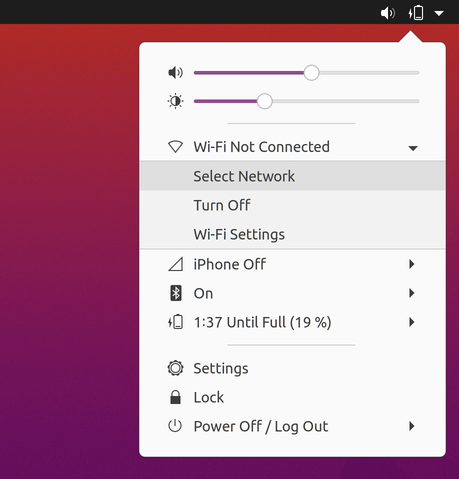
\includegraphics[width=0.0truein]{wifi1.png}
\caption{}

\end{figure}

\begin{figure}[h]{}
\centering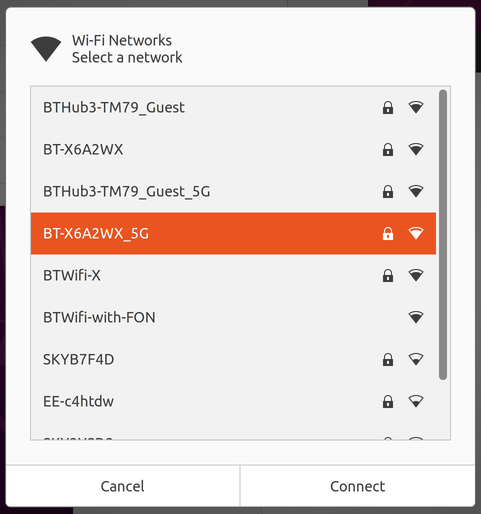
\includegraphics[width=0.0truein]{wifi2.png}
\caption{}

\end{figure}

\begin{figure}[h]{}
\centering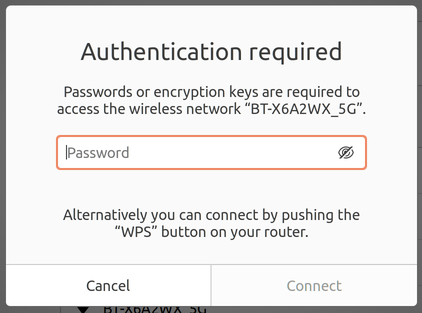
\includegraphics[width=0.0truein]{wifi3.png}
\caption{}

\end{figure}

\begin{figure}[h]{}
\centering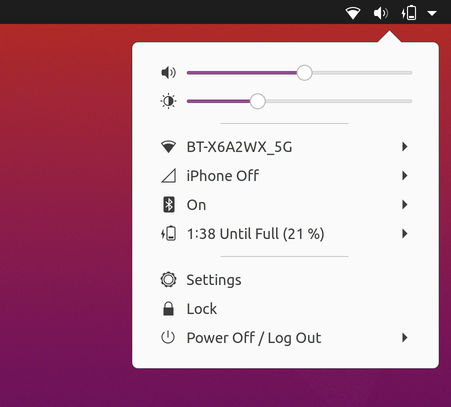
\includegraphics[width=2.5truein]{wifi4.png}
\caption{}

\end{figure}

\hypertarget{x-ios}{\subsubsection*{iOS}}
Connection to a network in iOS is similarly easy, requiring the usage of the Settings app. The Settings app contains a "Wi-Fi" submenu, that can be used for network discovery and connection. It also stores previous connection information, shows connection status, and has a toggle for WiFi overall.


\begin{figure}[h]{}
\centering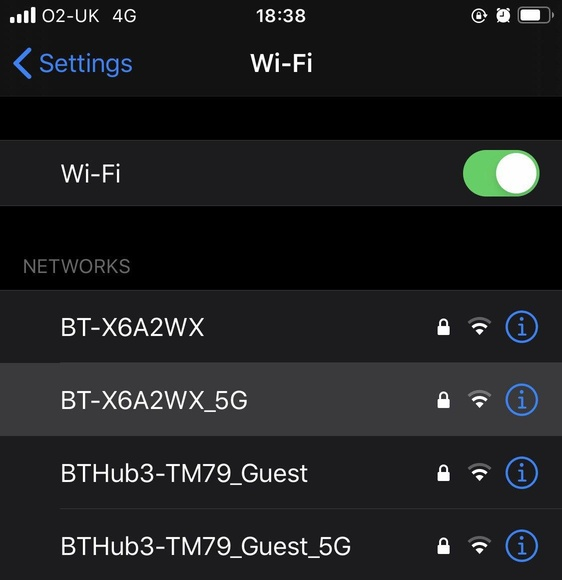
\includegraphics[width=2.5truein]{iphonewifi1.jpg}
\caption{}

\end{figure}

\begin{figure}[h]{}
\centering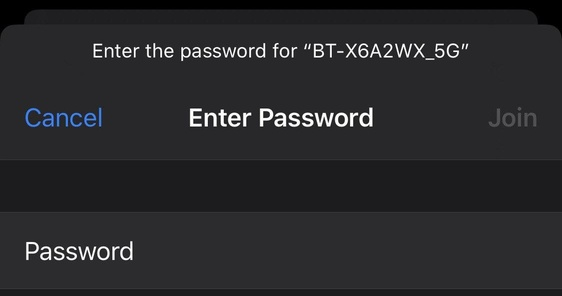
\includegraphics[width=2.5truein]{iphonewifi2.jpg}
\caption{}

\end{figure}

\begin{figure}[h]{}
\centering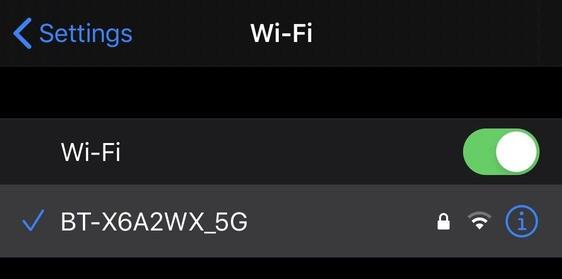
\includegraphics[width=2.5truein]{iphonewifi3.jpg}
\caption{}

\end{figure}

\hypertarget{x-nintendo-switch}{\subsubsection*{Nintendo Switch}}
The system settings app has an Internet tab for wired and wireless network info.


\begin{figure}[h]{}
\centering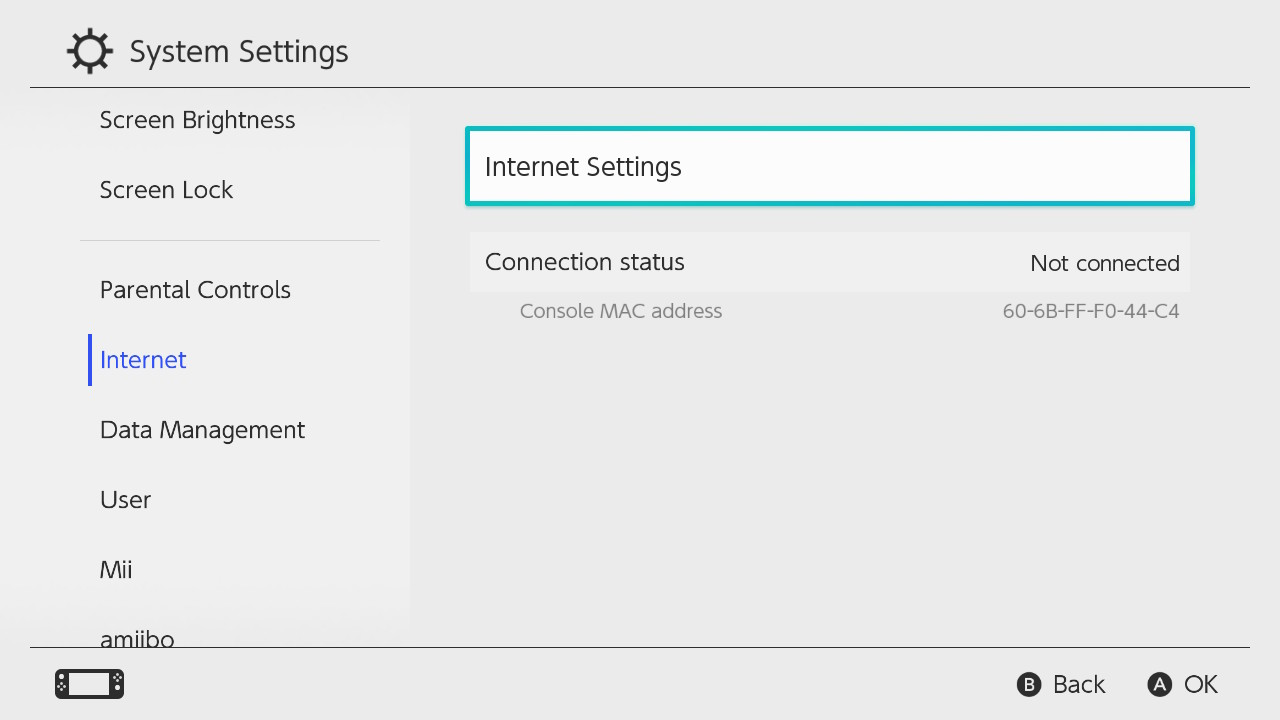
\includegraphics[width=2.5truein]{wifiswitch1.jpg}


\end{figure}

This section discovers nearby networks for configuration.


\begin{figure}[h]{}
\centering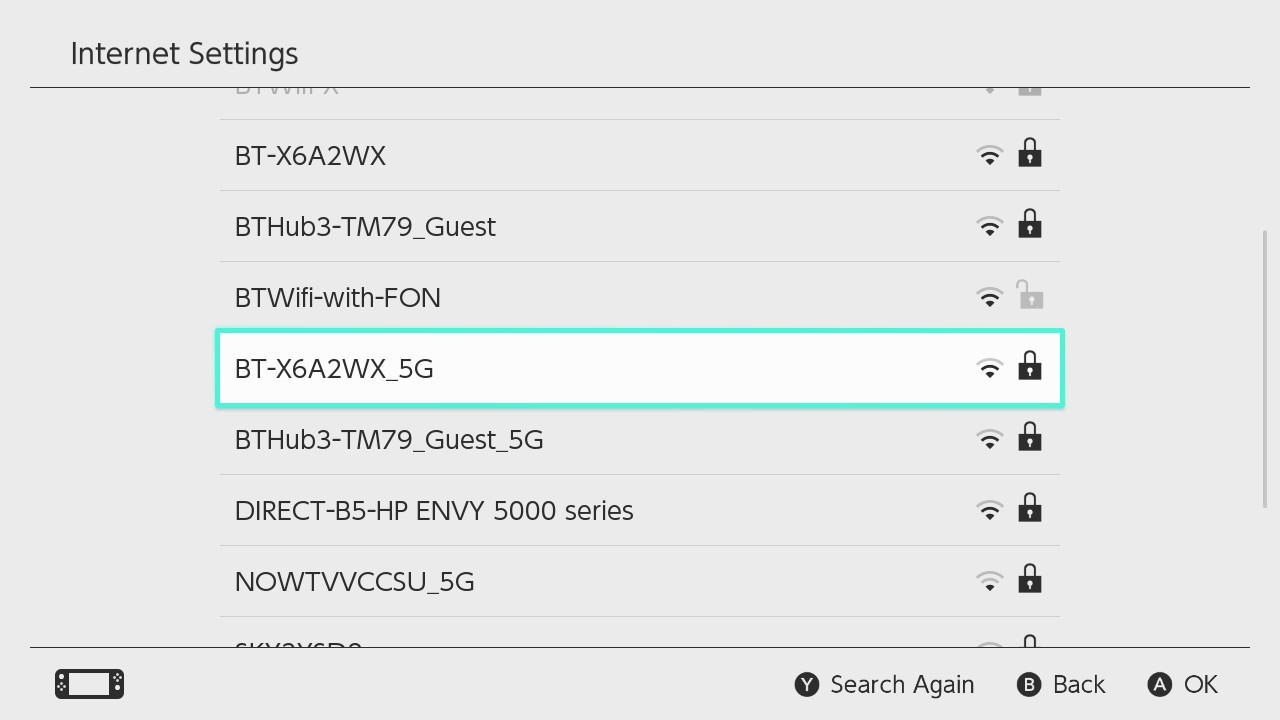
\includegraphics[width=2.5truein]{wifiswitch2.jpg}


\end{figure}

Once the password has been entered, the system test-connects to Nintendo servers.


\begin{figure}[h]{}
\centering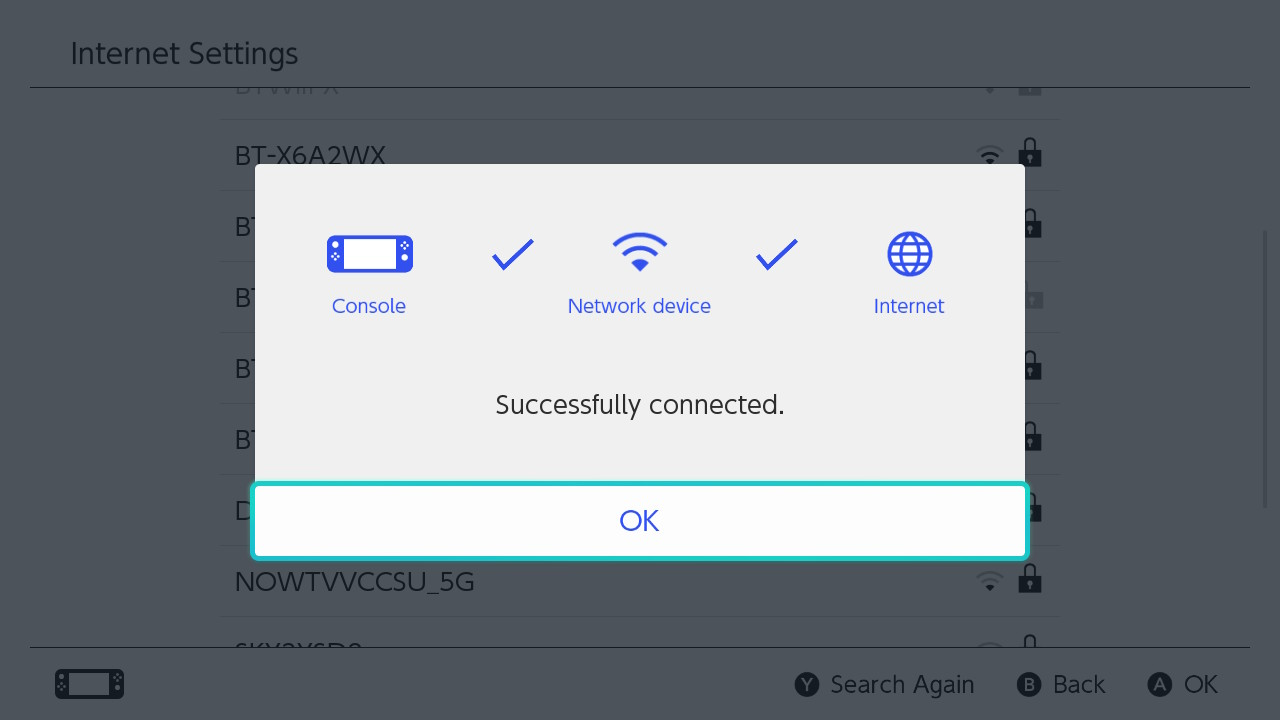
\includegraphics[width=0.0truein]{wifiswitch3.jpg}


\end{figure}

The Internet tab now shows various info about the connection status, including the IP.


\begin{figure}[h]{}
\centering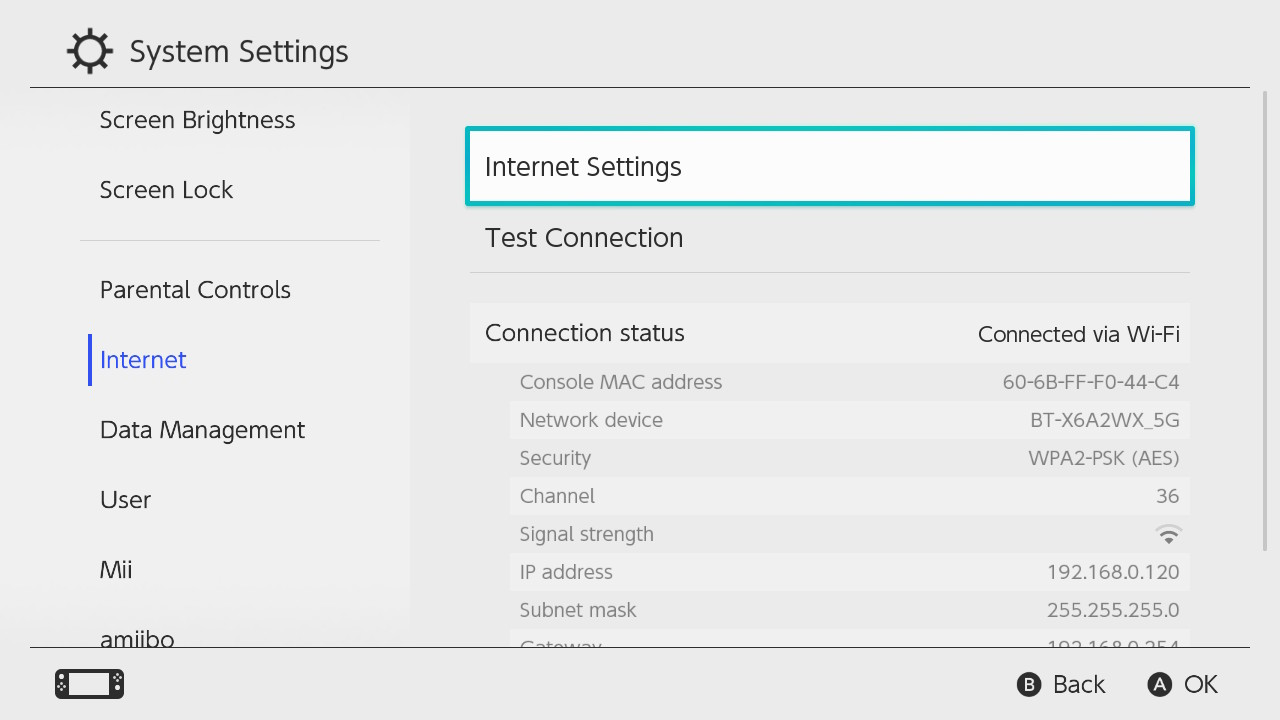
\includegraphics[width=0.0truein]{wifiswitch4.jpg}


\end{figure}

\hypertarget{x-testing-the-connection}{\subsection*{Testing the Connection}}
The Nintendo Switch settings app shows information about the network connection which can be utilised to test the network connection between two devices. This information can be found out on other devices through multiple methods, but it is usually easiest to use the same utility that is used for conection.


\begin{figure}[h]{}
\centering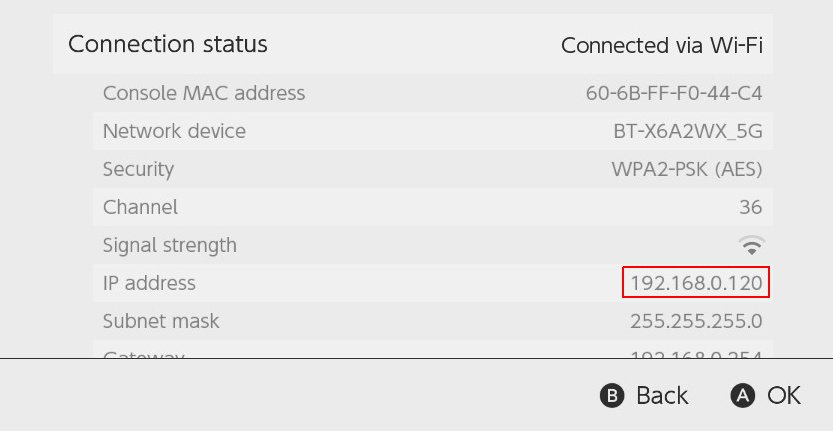
\includegraphics[width=2.5truein]{wifiswitch5.jpg}
\caption{}

\end{figure}

The \texttt{ping} command shows various information on returned pings, the most significant of which being the latency (time). A lack of responses indicates that the target address is unreachable.


\begin{figure}[h]{}
\centering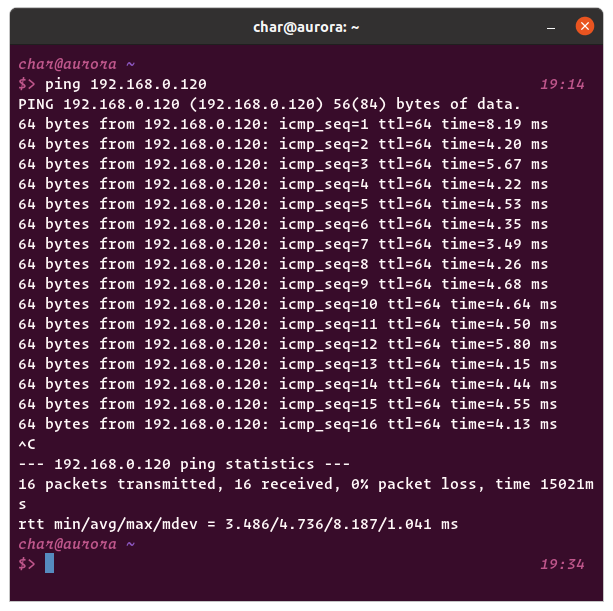
\includegraphics[width=2.5truein]{pingterminal.png}
\caption{}

\end{figure}

As well as this, the network connection to the greater internet can be tested using \texttt{wget}. This type of test relies on a known-working network address, for which something like \texttt{google.com} is a good example due to infrequent downtime.


\begin{figure}[h]{}
\centering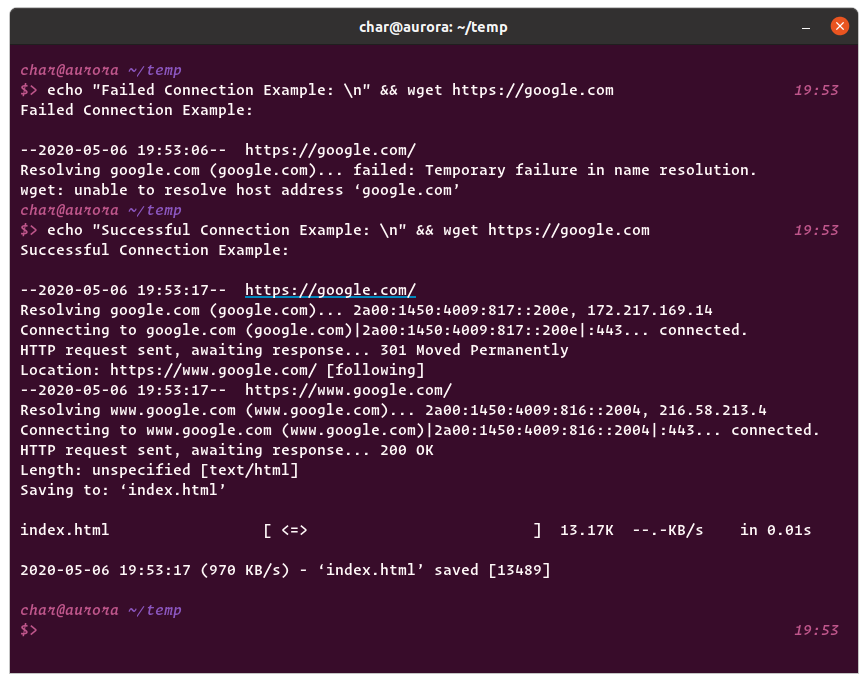
\includegraphics[width=2.5truein]{wget.png}
\caption{}

\end{figure}

\hypertarget{x-troubleshooting-research-tasks}{\section*{Troubleshooting Research Tasks}}
\hypertarget{x-dell-inspiron-530}{\subsection*{Dell Inspiron 530}}
\admonition{NOTE}{A Dell Inspiron 530 is having problems powering up. When trying to turn the machine on, the computer gives 6 short beeps, waits and then repeats this. Nothing is displayed on the screen.}
According to Dell’s support article for desktop beep-codes, 6 short beeps, a gap, then repetition implies Beep Code 6. This beep code is described as "Video BIOS", and relates to a video card fault or chip failure cite:[Dell1]. Dell’s recommended solution is to resolve the hardware issue with a built-in or online diagnostic cite:[Dell1], however my suggestion would be to replace the GPU (provided it’s not integrated into the CPU) in the system as the first step in troubleshooting.


\hypertarget{x-windows-update-has-failed}{\subsection*{Windows Update has failed}}
\admonition{NOTE}{Windows Update has failed with an error code of 0x8007000e.}
This update error code can occur with feature updates on Windows, commonly with distortion appearing on-screen during the update. This could have many causes, the most likely of which relates to problems with the video card and OS integration. According to online forums, there are a few things that can be done which can contribute to fixing this issue:


\begin{itemize}

\item Making sure that video drivers are up to date, and correctly installed

\item Performing a BIOS update and trying again

\item Installing the update from an ISO installer

\end{itemize}


The last solution writes over the existing operating system while retaining user settings and data, which means that the issue of updating can’t occur, as nothing is being 'updated'. Even so, it’s a complex solution for an issue that may be solved by the other steps cite:[MSupport1] cite:[MSupport2].


\hypertarget{x-slow-and-intermittent-wifi}{\subsection*{Slow and intermittent WiFi}}
\admonition{NOTE}{Your WiFi network connection appears slow and intermittent. You think there might be some kind of signal issue. Give troubleshooting steps.}
There are a few factors that contribute to WiFi connections being slow or intermittent, with multiple solutions for stability and speed. These include:


\hypertarget{x-signal-strength}{\subsubsection*{Signal Strength}}
The most obvious problem relating to connection issues is to do with signal strength. This issue usually relates to the distance from the access point, though it can also be an issue if there are certain materials between the client and the access point: thick concrete, for example, can inhibit a WiFi signal and cause issues.


This can be solved through better positioning of wireless access points and home routers, placing them centrally in the area of intended use, and having wireless repeaters should the area be too large or have blockages cite:[cnet1].


\hypertarget{x-signal-interference}{\subsubsection*{Signal Interference}}
Similar to signal strength, interference can impact WiFi signals significantly, lowering the signal-to-noise ratio, making the connection slow or unstable. This issue is most common in built up areas, with various WiFi bands being used up by other people in the local area. This occurs most commonly in the 2.4GHz range due to the penetration of the signal, with the 5GHz range being less congested but having a lower range cite:[Is5Ghz].


This can be solved by switching all home routers, repeaters, and access points to use a less congested band in either the 2.4GHz range or preferably the 5GHz range, if possible cite:[cnet1].


\hypertarget{x-bandwidth}{\subsubsection*{Bandwidth}}
Depending on the quantity of users on the network, bandwidth could be a consideration for slow or intermittent WiFi. If other users have particularly high network demands, like with streaming or general downloading, all the bandwidth could be used up. The solution for this issue relates to freeing up this bandwidth, if possible, by making sure that all unnecessary devices or processes are shut off. Additionally, security can impact bandwidth usage, with unsecured networks potentially having people leech bandwidth cite:[cnet1].


\hypertarget{x-isp-related-issue}{\subsubsection*{ISP Related Issue}}
Sadly, not all issues relating to networking connections can be solved on-site. Networking infrastructure upstream from a household or business can fail, requiring the ISP to resolve any issues involved. Long-term issues can also arise, like faulty cabling, that can take lots of time for an ISP to fix. Sadly, there’s no reliable solution for this kind of issue outside of changing ISP, if possible cite:[cnet1].


\hypertarget{x-pc-hardware-maintenance}{\section*{PC Hardware Maintenance}}
\hypertarget{x-step-1:-cpu-heatsink}{\subsection*{Step 1: CPU Heatsink}}
My CPU Fan is in a pull configuration, meaning the heatsink is easily accessed to clean. The right-side of the heatsink in this image is where the dust would collect, with the fan on the left side pulling air through the fins. This configuration is preferential to a fan that pushes air through, as the fan would need to be removed in order for dust to be cleaned out.


\begin{figure}[h]{}
\centering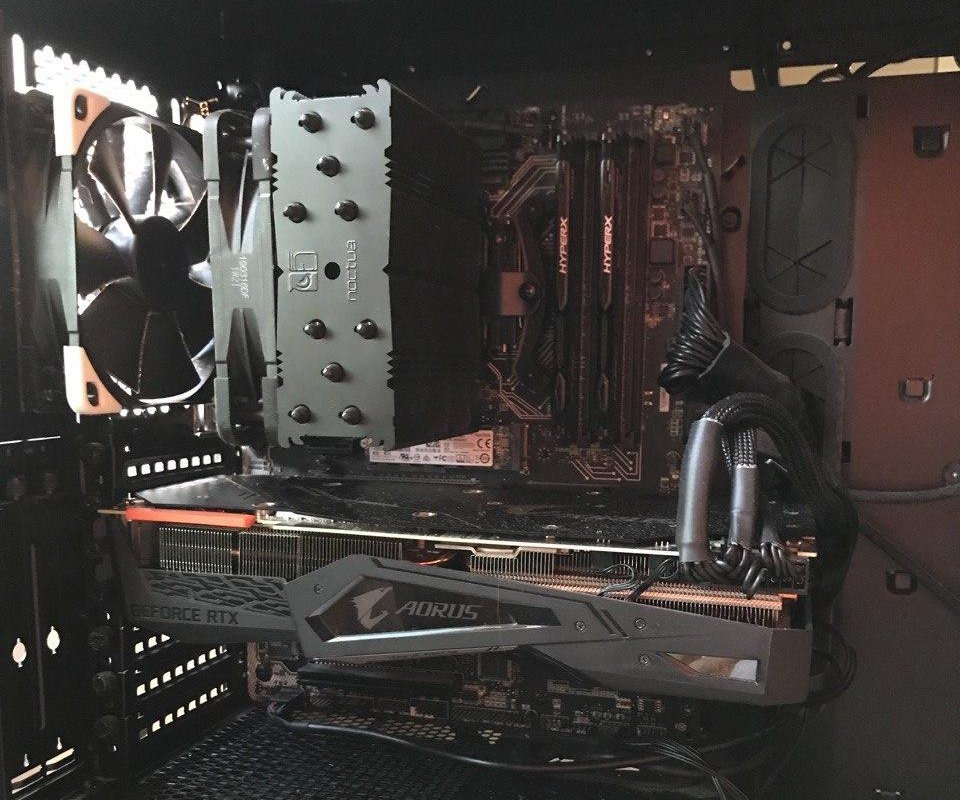
\includegraphics[width=2.5truein]{10.jpg}
\caption{}

\end{figure}

\hypertarget{x-step-2:-gpu-heatsink}{\subsection*{Step 2: GPU Heatsink}}
The GPU power, output cables, and screws need to be removed in order to access the GPU’s heatsink for cleaning. Since the card’s cooler is an open design, access to the fins is relatively easy when compared with blower-style coolers. This being said, the card didn’t require any cleaning in this instance.


\begin{figure}[h]{}
\centering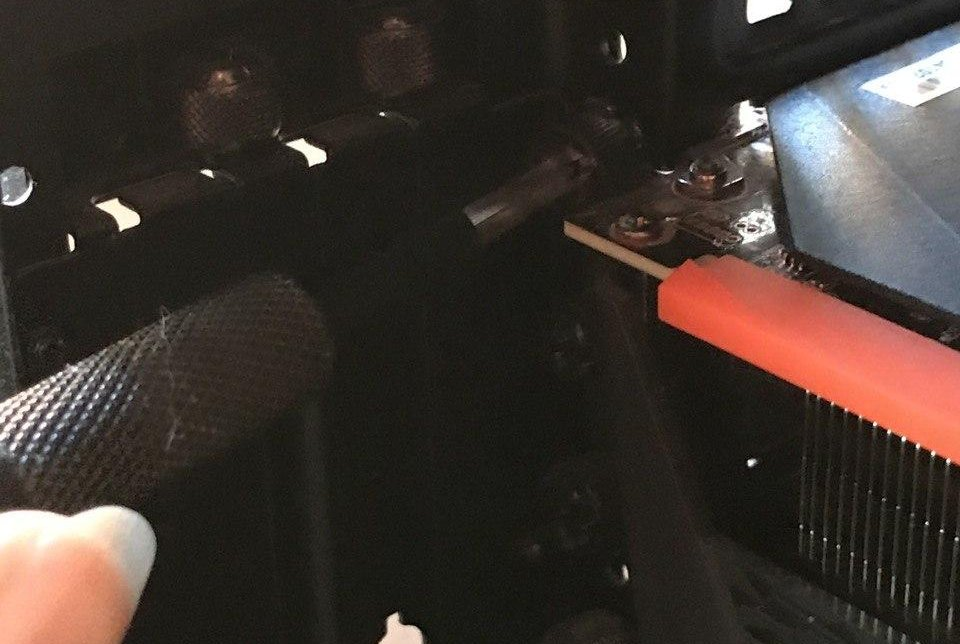
\includegraphics[width=2.5truein]{3.jpg}
\caption{}

\end{figure}

\begin{figure}[h]{}
\centering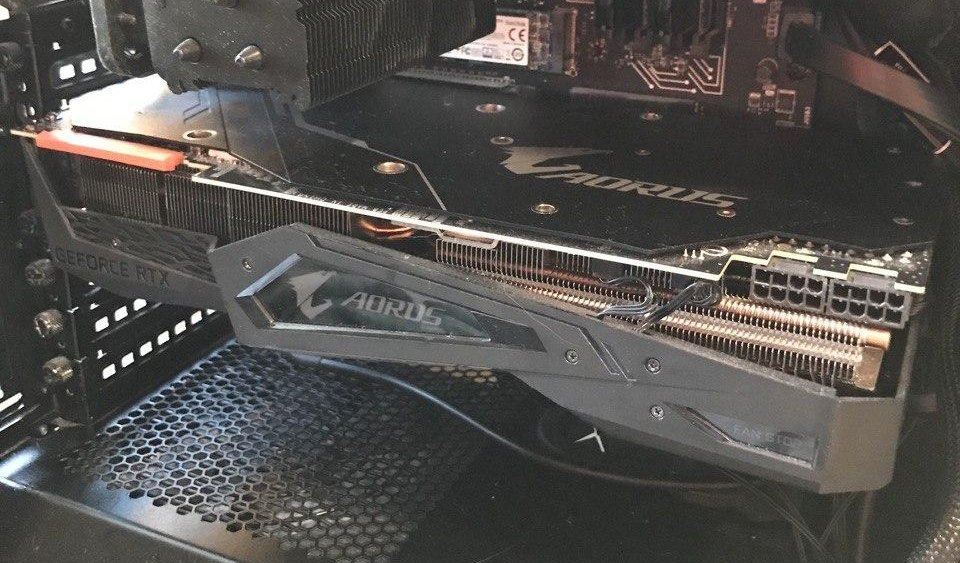
\includegraphics[width=2.5truein]{5.jpg}
\caption{}

\end{figure}

\begin{figure}[h]{}
\centering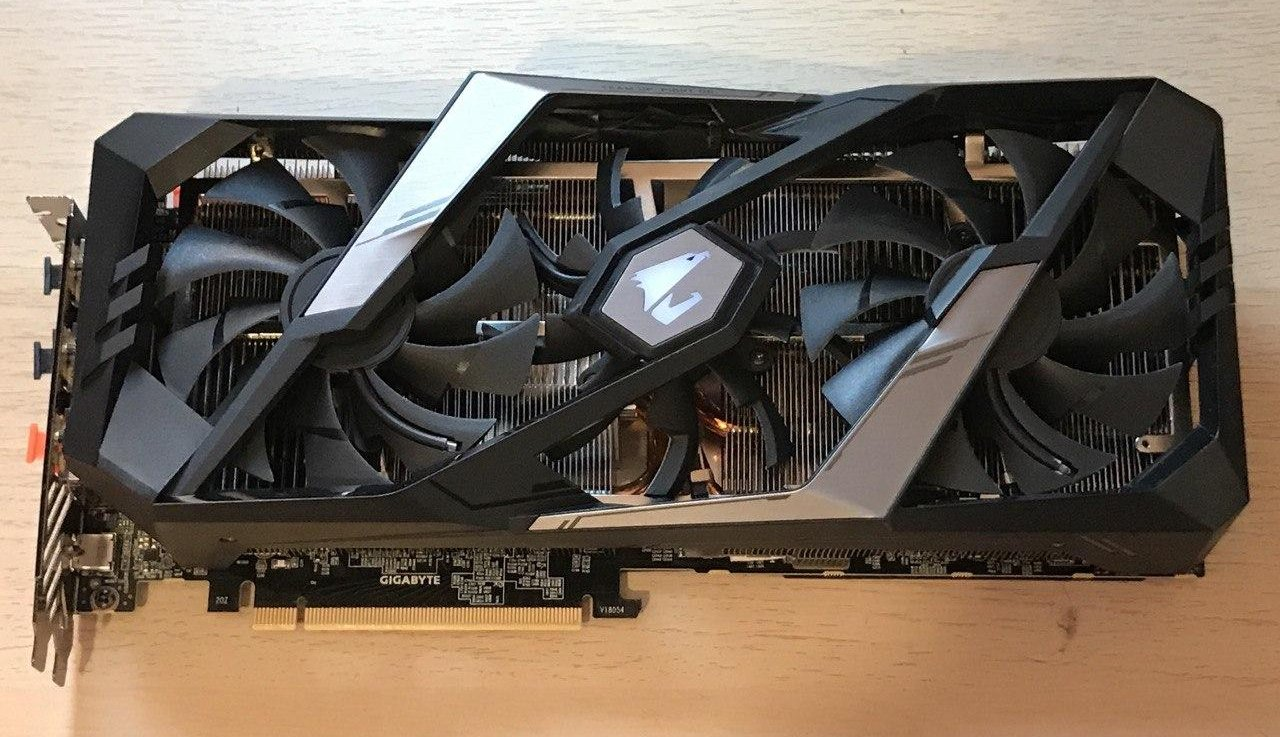
\includegraphics[width=2.5truein]{4.jpg}
\caption{}

\end{figure}

\hypertarget{x-step-3:-front-dust-filter}{\subsection*{Step 3: Front Dust Filter}}
The front dust filter for this case is magnetic and easily removed by swinging out the side-panel for access. This filter captures the majority of the dust entering the system, with barely any dust on the internal components in comparison. This is by far the messiest section of maintenance, with the best solution involving taking the filter outside to dispose of dust.


\begin{figure}[h]{}
\centering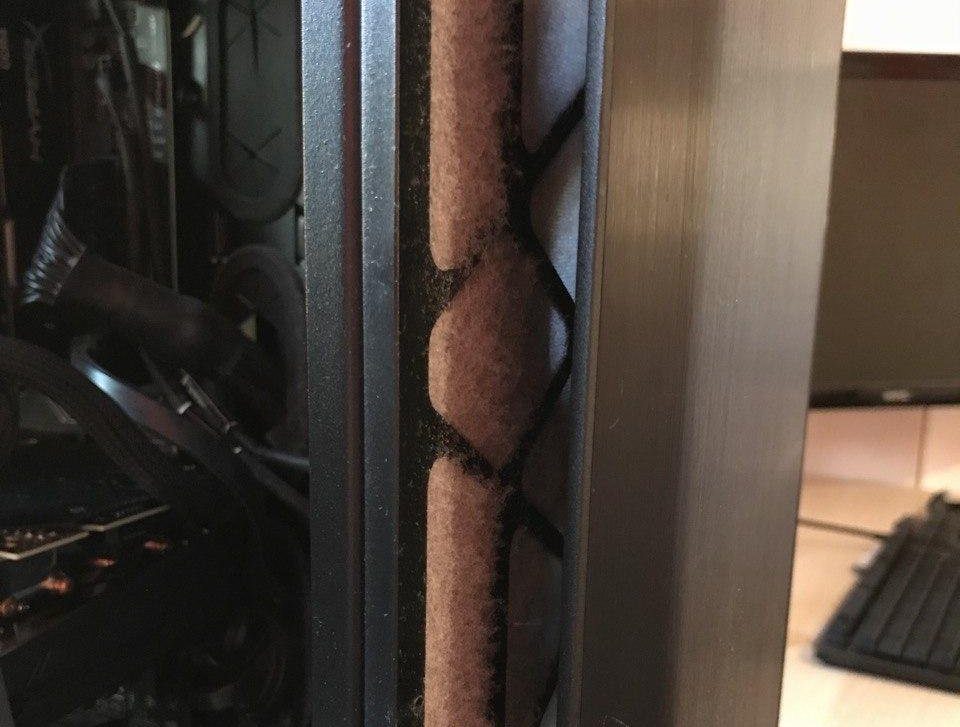
\includegraphics[width=2.5truein]{6.jpg}
\caption{}

\end{figure}

\hypertarget{x-step-4:-psu-dust-filter}{\subsection*{Step 4: PSU Dust Filter}}
This case also features a dust filter for the Power Supply Unit (PSU), allowing for easy cleaning. In this case, the dust-filter is clear due to the PC being placed on top of a desk during normal operation.


\begin{figure}[h]{}
\centering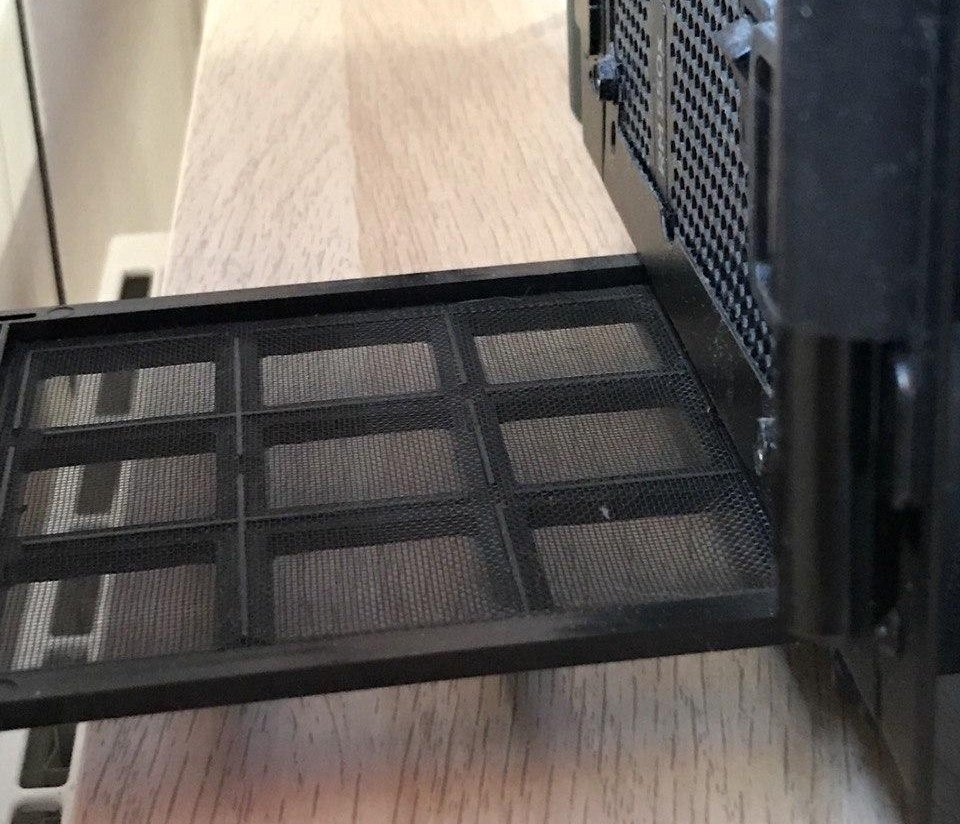
\includegraphics[width=0.0truein]{8.jpg}
\caption{}

\end{figure}

\hypertarget{x-step-5:-internal-dusting}{\subsection*{Step 5: Internal Dusting}}
While the front panel dust filter is extremely effective, finer dust can make it through, landing on the internal components, case surfaces, and case fans. These fans shown are at the front of the case, pulling air in, and have minor levels of dust. Additionally, the panel behind these fans has some light dust too.


\begin{figure}[h]{}
\centering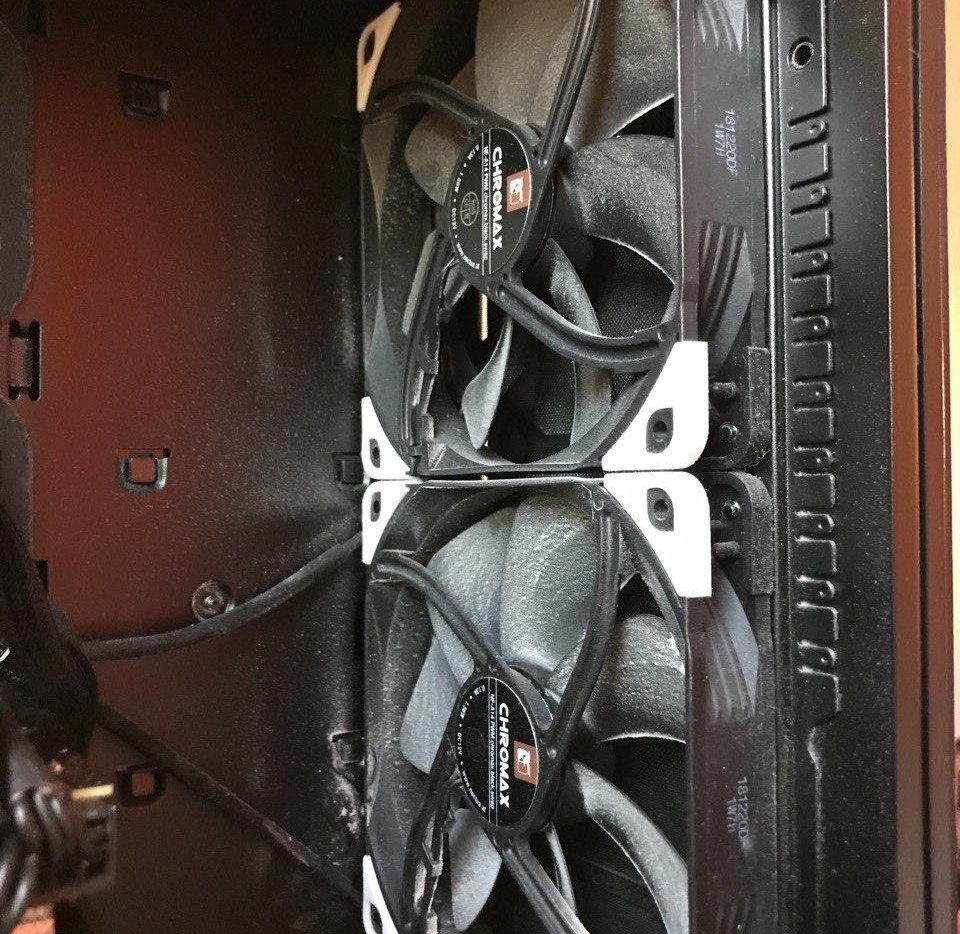
\includegraphics[width=0.0truein]{9.jpg}
\caption{}

\end{figure}

\hypertarget{x-pc-software-maintenance}{\section*{PC Software Maintenance}}
Software maintenance on Ubuntu has two major methods. The command line (bash) can be used in conjunction with APT (Advanced Package Tool), the primary package manager for the distribution, to update and clean up packages on the system. Additionally, Ubuntu includes software designed to simplify basic software maintenance for end-users, derived from Gnome. While simpler, this software can perform most of the essential maintenance required for a system.


\hypertarget{x-ubuntu-(gnome)-software}{\subsection*{Ubuntu (Gnome) Software}}
\hypertarget{x-disks-(\texttt{gnome-disk-utility})}{\subsubsection*{Disks (\texttt{gnome-disk-utility})}}
The application \texttt{gnome-disk-utility} is designed to manage disks and partitions, with functionality for formatting, disk imaging, benchmarking, SMART self-tests, and filesystem checks/repair. This functionality can be used to analyse hard drives, ranging from Solid State memory to Flash memory. The partitions can be checked for errors using this utility, however


\admonition{WARNING}{Any partition has to be checked while it is unmounted; This means that a live-usb should be used for checking the host filesystem, as it cannot be unmounted while the computer is booted from it.}
\begin{figure}[h]{}
\centering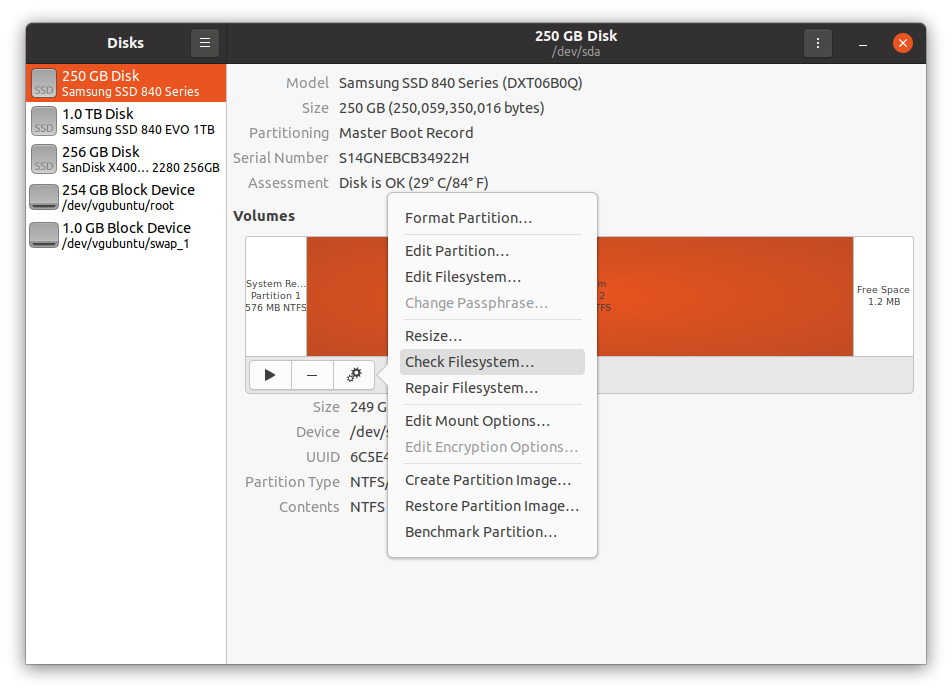
\includegraphics[width=2.5truein]{CheckFilesystem.png}
\caption{}

\end{figure}

\begin{figure}[h]{}
\centering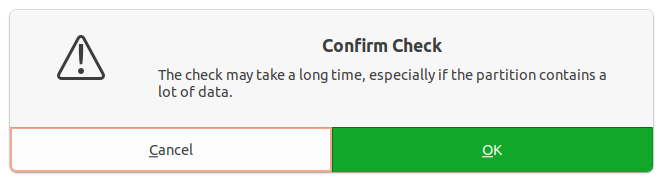
\includegraphics[width=2.5truein]{CFConfirmation.png}
\caption{}

\end{figure}

\begin{figure}[h]{}
\centering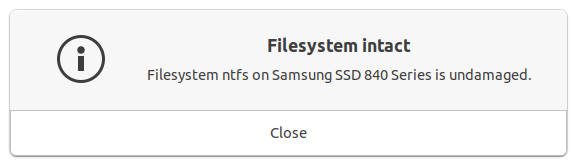
\includegraphics[width=2.5truein]{CFResult.png}
\caption{}

\end{figure}

\hypertarget{x-settings-(\texttt{gnome-settings})}{\subsubsection*{Settings (\texttt{gnome-settings})}}
The \texttt{gnome-settings} app can clear temporary files and the rubbish folder. This process can be automated, with the settings shown on the user interface screenshot depicting


\begin{figure}[h]{}
\centering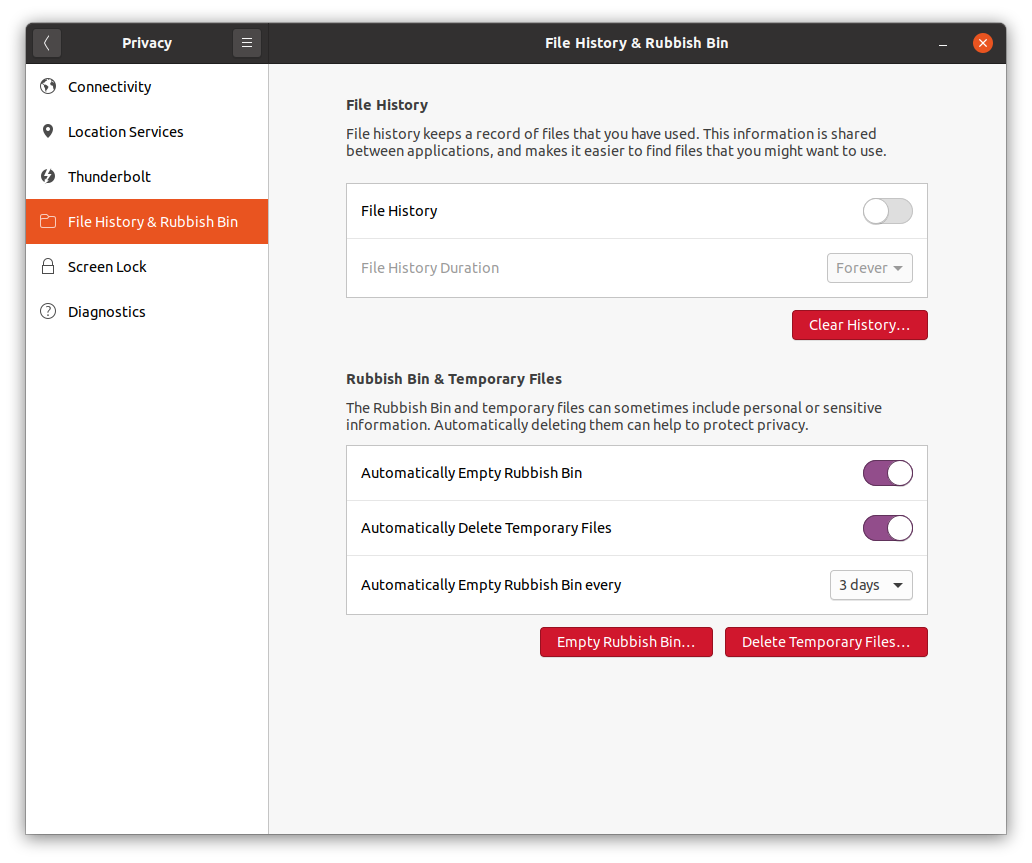
\includegraphics[width=2.5truein]{SettingsStorage.png}
\caption{}

\end{figure}

\begin{figure}[h]{}
\centering
\includegraphics[width=2.5truein]{SettingsRubbish.png}
\caption{}

\end{figure}

\begin{figure}[h]{}
\centering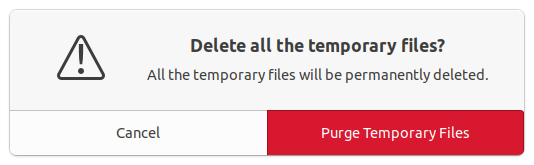
\includegraphics[width=2.5truein]{SettingsTemp.png}
\caption{}

\end{figure}

\hypertarget{x-command-line}{\subsection*{Command Line}}
As described earlier, APT is the core system by which Debian manages packages. Using apt, it’s possible to perform multiple operations that contribute towards the maintenance of a PC’s software, primarily involving cleaning out old packages and updating packages. This image shows the set of commands that are involved with this process.


\begin{figure}[h]{}
\centering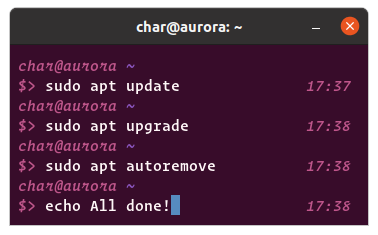
\includegraphics[width=2.5truein]{CommandShowcase.png}


\end{figure}

\begin{itemize}

\item \texttt{apt update} refreshes the package index from the apt sources on the system.

\item \texttt{apt upgrade} updates existing packages, should updates be available.

\item \texttt{apt autoremove} cleans up packages that are no longer needed.

\end{itemize}


(For the purposes of this log, \texttt{apt} is replaced with \texttt{apt-get} which, while identical in functionality, doesn’t have any issues with terminal history. Additionally, some repeated lines have been removed for conciseness)


\begin{verbatim}
char@aurora ~
$> sudo apt-get update

Hit:1 http://gb.archive.ubuntu.com/ubuntu focal InRelease
...
Get:15 http://gb.archive.ubuntu.com/ubuntu focal-backports/universe amd64 DEP-11 Metadata [528 B]
Fetched 423 kB in 1s (662 kB/s)
Reading package lists... Done

char@aurora ~
$> sudo apt-get upgrade

Reading package lists... Done
Building dependency tree
Reading state information... Done
Calculating upgrade... Done
The following packages will be upgraded:
  python3-update-manager strace update-manager update-manager-core
4 to upgrade, 0 to newly install, 0 to remove and 0 not to upgrade.
Need to get 979 kB of archives.
After this operation, 98.3 kB of additional disk space will be used.
Do you want to continue? [Y/n]
Get:1 http://gb.archive.ubuntu.com/ubuntu focal-updates/main amd64 python3-update-manager all 1:20.04.10 [36.5 kB]
Get:2 http://gb.archive.ubuntu.com/ubuntu focal-updates/main amd64 update-manager-core all 1:20.04.10 [11.3 kB]
Get:3 http://gb.archive.ubuntu.com/ubuntu focal-updates/main amd64 update-manager all 1:20.04.10 [551 kB]
Get:4 http://gb.archive.ubuntu.com/ubuntu focal-updates/main amd64 strace amd64 5.5-3ubuntu1 [380 kB]
Fetched 979 kB in 1s (1,208 kB/s)
(Reading database ... 264637 files and directories currently installed.)
Preparing to unpack .../python3-update-manager_1%3a20.04.10_all.deb ...
Unpacking python3-update-manager (1:20.04.10) over (1:20.04.9) ...
...
Preparing to unpack .../strace_5.5-3ubuntu1_amd64.deb ...
Unpacking strace (5.5-3ubuntu1) over (4.26-0.2ubuntu3) ...
Setting up strace (5.5-3ubuntu1) ...
...
Processing triggers for man-db (2.9.1-1) ...

char@aurora ~
$>sudo apt-get autoremove

Reading package lists... Done
Building dependency tree
Reading state information... Done
The following packages will be REMOVED
  fonts-lato libruby2.7 rake ruby ruby-minitest ruby-net-telnet ruby-paint
  ruby-power-assert ruby-test-unit ruby-trollop ruby-xmlrpc ruby2.7
  rubygems-integration
0 to upgrade, 0 to newly install, 13 to remove and 0 not to upgrade.
After this operation, 30.8 MB disk space will be freed.
Do you want to continue? [Y/n]
(Reading database ... 229902 files and directories currently installed.)
Removing fonts-lato (2.0-2) ...
dpkg: warning: while removing fonts-lato, directory '/usr/share/fonts/truetype/lato' not empty so not removed
Removing ruby-trollop (2.0-2) ...
...
Removing rubygems-integration (1.16) ...
Processing triggers for libc-bin (2.31-0ubuntu9) ...
Processing triggers for man-db (2.9.1-1) ...
Processing triggers for fontconfig (2.13.1-2ubuntu3) ...

char@aurora ~
$>echo All done!

All done!
\end{verbatim}

Following this, the sources are checked for new package updates, all packages are upgraded, and all redundant packages are removed.


\hypertarget{x-references}{\section*{References}}
bibliography::[]


\end{document}

